\section{Abfahrtspläne}
\todo{Deadline: 22.06.}
\todo{Abgrenzung des Begriffes ''Abrfahrtsplan'' vom Begriff ''Fahrplan''. Wir nutzen Abfahrtspläne, da wir nur den Abfahrtszeitpunkt eines Zuges kennen. Die restlichen Zeitpunkte ergeben sich aus der Simulation. Im Anschluss erläutere ich die drei Arten von Abfahrtsplänen, die wir verwenden.}

Zur Abgrenzung von dem Begriff Fahrplan wird hier der Begriff \emph{Abfahrtsplan} eingeführt. Im Gegensatz zu einem Fahrplan enthälkt ein Abfahrtsplan lediglich folgende Informationen:
\begin{itemize}
    \item Die Zuggattung (Im Folgenden Zugtyp genannt)
    \item Die Abfahrtszeiten an der Starthaltestelle
    \item Eine Liste der Zwischenhaltestellen und die Endhaltestelle jedoch keine Ankunfts- oder Abfahrtzeiten
\end{itemize}
Da die Ankunfts- und Abfahrtzeiten Teil der Ergebnisse sind, die die Simulation produziert, können Fahrpläne nicht als Eingabe dienen. Daher verwenden wir Abfahrtspläne. Wie bereits in den Anforderungen angedeutet, werde drei verschiedene Arten von Abfahrtsplänen benötigt. Solche die zeitlich regelmäßge Zugfahrten beschreiben (Regelmäßige Abfahrtspläne), solche die Zugfahrten mit zufälligen Abfahrtszeiten beschreiben (Zufällige Abfahrtspläne) und solche, deren Abfahrtzeiten sich nach einem historischen Kohlebadarf richten (Bedarfsorientierte Abfahrtspläne). Jeder Abfahrtsplan besitzt eine Startzeit ($t_s \in \mathbb{N}$) und eine Endzeit ($t_e \in \mathbb{N}$), jeweils in Sekunden. $t_s$ beschreibt den Zeitpunkt in der Simulation, wenn der Abfahrtsplan aktiv wird, $t_e$ beschreibt den Zeitpunkt, wenn der Abfahrtsplan deaktiviert wird. Für jede Abfahrtszeit eines Zuges $t_a$ gilt also $t_s\leq t_a \leq t_e$. Die Details der drei Varianten werden im Folgenden erklärt.

\subsection{Regelmäßige Abfahrtspläne}

Der regelmäßige Abfahrtsplan beschreibt die Abfahrt von Zügen in regelmäßigen zeitlichen Abständen und dient der Modellierung von klassischen fahrplan-basiertem Verhalten. Er besitzt eine Periode $p\in\mathbb{N}$ in Sekunden, welche die Größe des zeitlichen Abstandes angibt. Ein regelmäßiger Abfahrtsplan lässt somit Züge zu den Zeitpunkten $t_a=t_s+np$ mit $n\in\mathbb{N}$ abfahren.

\subsection{Zufällige Abfahrtspläne}

Der regelmäßige Abfahrtsplan beschreibt die Abfahrt von Zügen in zufälligen zeitlichen Abständen. Er dient damit der Modellierung von Zügen, die unplanmäßig oder unvorhergesehen kurzfristig fahren. Dieser Abfahrtsplan besitzt eine Wahrscheinlichkeitsverteilung $P$, die angibt, mit welcher Häufigkeit ein Züge in einer bestimmten Zeitspanne abfahren. $P$ folgt einer Gleichverteilung. Die Wahrscheinlichkeit für eine Abfahrt ist also zu jedem Zeitpunkt gleich.

\subsection{Bedarfsorientierte Abfahrtspläne}

Der bedarfsorientierte Abfahrtsplan beschreibt die Abfahrt von Zügen in zeitlichen Abständen, die sich nach einem historischen Kohlebedarf richten. Er dient damit der Modellierung von Kohlezügen. Dieser Abfahrtsplan besitzt eine Kohlebedarfsfunktion $k:\mathbb{N}\to\mathbb{R}$, die angibt, wie viel Kohle in Abhängigkeit von der Zeit $t$ benötigt wird. Sie ergibt sich aus den historischen Kohlebedarfsdaten. Weiterhin existieren der Zeitpunkt $t_0 \in \mathbb{N}$ in Sekunden, an welchem die historischen Daten beginnen und die Zeitspanne $t_r \in \mathbb{N}$ in Sekunden, welche die zeitliche Auflösung der Daten angibt. Weiterhin ist $c\in\mathbb{R}$ die Menge an Kohle, die ein Kohlezug transportieren kann. Zur Berechnung der Abfahrtszeiten wird zunächst die Funktion $a: \mathbb{N} \to \mathbb{R}$ aufgestellt, die den akkumulierten Kohlebedarf zum Zeitpunkt $t$ seit $t_0$ berechnet (siehe Formel \ref{eq:kohle-accu}). Dabei ist $n\in\mathbb{N}$ die Anzahl der Datenpunkte.

\begin{equation}
    a(t)=\sum_{i=0}^n  k(t_ri+t_0)\label{eq:kohle-accu}
\end{equation}

Der Abfahrtsplan soll nun stets dann Züge abfahren lassen, wenn die Menge an Kohle, die transportiert werden muss, die Menge erreicht, die ein Zug transportieren kann. Die transportierte Menge wird dann von der bisher akkumulierten Menge abgezogen. Formel \ref{eq:kohle-fmod} stellt das dar.

\begin{equation}
    f(t, c)=fmod(a(t), c)\label{eq:kohle-fmod}
\end{equation}\footnote{Die Funktion $fmod:(\mathbb{R},\mathbb{R}) \to \mathbb{R}$ ist definiert als $(x,y)\mapsto x-ny$ mit $n\in\mathbb{Z}$, $x<0\Leftrightarrow fmod(x,y)<0$ und $fmod(x,y)<|y|$. Intuitiv formuliert, gibt die Funktion den Rest der Division $\frac{x}{y}$ zurück.}

Abbildung \ref{fig:demand-math} zeigt schematisch das Verhalten eine bedarfsorientierten Abfahrtsplans. $k(t)$ zeigt den (hier zur Vereinfachung konstanten) Kohlebedarf. $a(t)$ stellt den akkumulierten Kohlebedarf dar. $f(t,c)$ zeigt die akkumulierte Kohlemenge abzüglich der transportierten Kohlemenge. Die Abfahrtszeiten sind durch rote Pfeile markiert.

\begin{figure}[H]
	\centering
	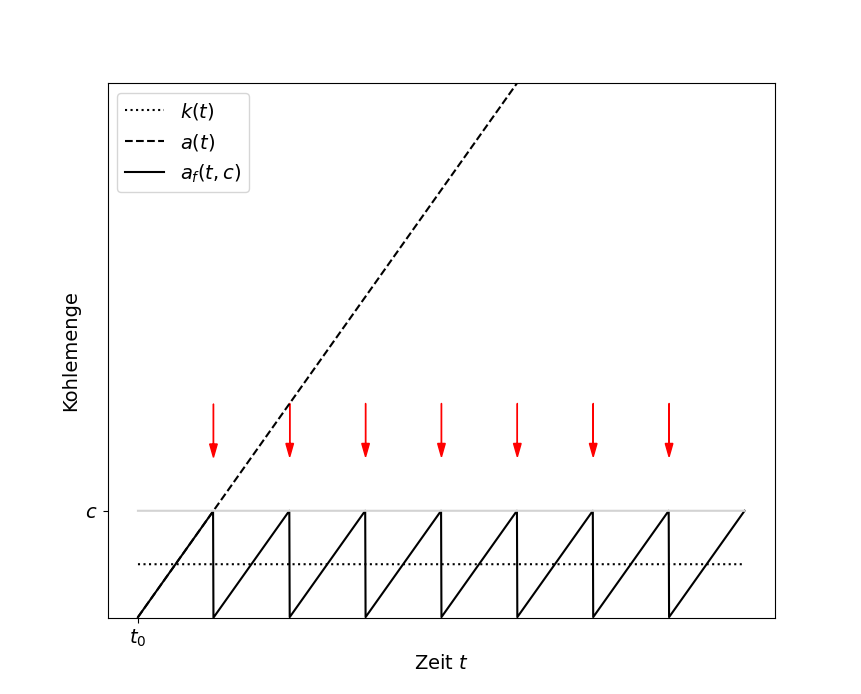
\includegraphics[width=1.0\linewidth]{images/demand-math.png}
	\caption{Schematisches Verhalten eines bedarfsorientierten Abfahrtsplans mit dem Kohlebedarf $k(t)$, dem akkumulierten Kohlebedarf $a(t)$ und der akkumulierten Kohlemenge abzüglich der transportierten Kohlemenge $f(t,c)$. Die roten Pfeile markieren die Abfahrtszeiten der Kohlezüge.}
	\label{fig:demand-math}
\end{figure}